% !TEX encoding = UTF-8
% !TEX TS-program = pdflatex
% !TEX root = ../tesi.tex

%**************************************************************
\chapter{Valutazione retrospettiva}
\label{cap:valutazione-retrospettiva}
%**************************************************************

\section{Difficoltà incontrate}
\label{sec:difficolta_incontrate}
Le prime difficoltà che ho incontrato sono state relative ai linguaggi: non avevo mai programmato in Dart e soprattutto non mi ero mai trovato a dover gestire la caratteristica che, quando innestato in Flutter, viene usato sia per le logiche di controllo che per produrre componenti grafiche dell'interfaccia utente. A questo si è aggiunta la necessità di dover usare altri tre linguaggi per le implementazioni native, ovvero Java e Kotlin per il lato Android e Swift per la parte iOS, che ho poi dovuto mettere in comunicazione diretta con Flutter (e nel caso di Java e Kotlin anche tra di loro).\\ 
Ho quindi speso una buona parte dello \textit{stage} a comprendere e gestire la grande varietà di linguaggi diversi.

\begin{figure}[H]
  \centering
  %\includegraphics[height=5cm]{screen_mobilesyn}
  
\includegraphics[width=.5\textwidth]{asa_google_search}\hfill
  
\includegraphics[width=.5\textwidth]{flutter_google_search}\\
  
\includegraphics[width=1\textwidth]{asa_flutter_google_search}
  \caption[Ricerca esatta Flutter e ASA 23 novembre]{Al 23 novembre 2022, una ricerca esatta di "flutter" mostra 87.5 milioni di risultati rilevanti, di "azure spatial anchors" 41 milioni mentre la combinazione delle due, solo 17}
\label{fig:search1}
\end{figure}

Le due problematiche che ritengo più rilevanti, però, sono state la mancanza di documentazione adeguata e la mancanza di supporto da parte della comunità degli sviluppatori.\\
Microsoft non fornisce un \textit{set} documentale adeguato per quanto riguarda \asa{}, mostrando il meno possibile della struttura interna (ad esempio come viene rappresentato un ancoraggio) e fornendo solo \api{} per effettuare operazioni ad alto livello (come il salvataggio in \textit{cloud} di un'\textit{anchor}), inoltre la ricerca della documentazione è macchinosa.\\
L'altro problema risiede nella difficoltà estrema di trovare supporto di terze parti (ad esempio in siti come \url{https://stackoverflow.com}), come mostro nelle figure \ref{fig:search1} e \ref{fig:search2}.

\begin{figure}[H]
  \centering
  %\includegraphics[height=5cm]{screen_mobilesyn}
  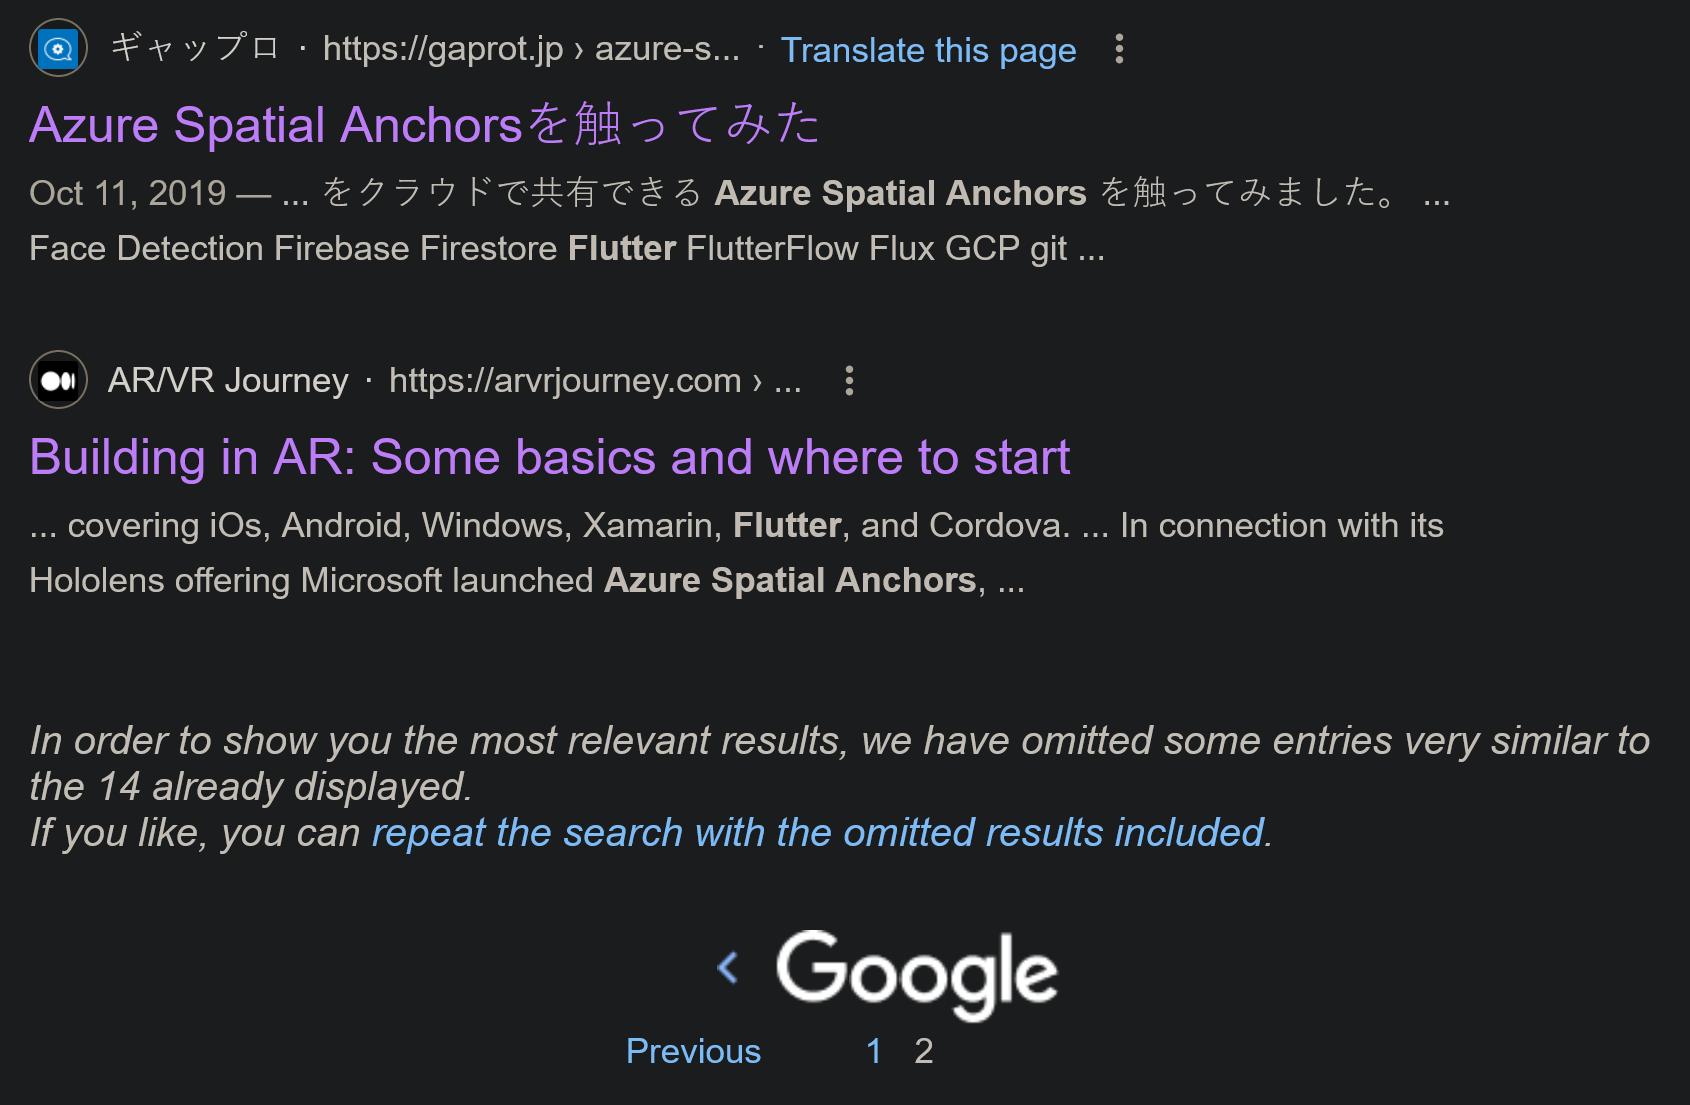
\includegraphics[width=.8\textwidth]{asa_flutter_search_today}
  \caption[Ricerca esatta Flutter e ASA 8 febbraio]{All'otto febbraio 2023 non si notano miglioramenti: solo 14 risultati rilevanti, alcuni in lingua giapponese, mostrano quando sia difficile trovare informazioni sull'argomento.}
  \label{fig:search2}
\end{figure}

Ho quindi dovuto, a causa di questa situazione, risolvere tutti i problemi incontrati senza poter fare affidamento su alcun aiuto esterno e questo ha esacerbato ulteriormente l'approccio \textit{trial-and-error} di cui si è parlato nella sezione \ref{sec:pianificazione}.

%************************************************************************************************************

\section{Raggiungimento obiettivi}
\subsection{Raggiungimento obiettivi proponente}
Riprendo quanto riportato in sezione \ref{sec:obiettivi} per trarre un bilancio sul grado di soddisfacimento dell'azienda nei confronti dei risultati ottenuti nel corso dello \textit{stage}, che schematizzo di seguito (riportando obiettivo, se è stato raggiunto e dove trovarne la prova).

\aCapo{}
\textbf{Obiettivi minimi:}

{
    \setlength{\freewidth}{\dimexpr\textwidth-10\tabcolsep}
    \renewcommand{\arraystretch}{1.5}
    \centering
    \setlength{\aboverulesep}{0pt}
    \setlength{\belowrulesep}{0pt}
    \rowcolors{2}{red!10}{white}
    \begin{longtable}{C{.8\freewidth} C{.162\freewidth} C{.115\freewidth}}
       \toprule
    \rowcolor{red}
    \textcolor{white}{\textbf{Obiettivo}}&
    \textcolor{white}{\textbf{Raggiunto}}&
    \textcolor{white}{\textbf{Fonte}}\\
    \toprule
    \endhead
    
    Studio e comprensione del linguaggio di programmazione Dart e del \textit{framework} Flutter & \cellcolor{green!20}SI & \ref{ch:flutter}\\
    Analisi strumenti Azure: Azure Console e \asa{}& \cellcolor{green!20}SI & \ref{subsec:azure}\\
    Ricerca di \textit{framework} e \sdk{} per implementare le \asa{} in Flutter& \cellcolor{green!20}SI & \ref{subsec:framework_ar}\\
    Eventuale studio di linguaggi necessari alle implementazioni native, come ad esempio Kotlin, Java, Unity o Swift & \cellcolor{green!20}SI & \ref{lst:android_channels}, \ref{lst:ios_channels}.\\
    Completamento del \textit{framework} scelto nell'app Flutter esistente& \cellcolor{green!20}SI &\ref{lst:mobilesyn_managers}, \ref{lst:arplug_manager} \\
    Completamento dello sviluppo dei componenti per rappresentare le \textit{anchor} nello spazio in realtà aumentata& \cellcolor{green!20}SI & \ref{lst:ar_view}\\
    Completamento dello sviluppo delle \api{} per l'interazione utente con gli ancoraggi in realtà aumentata& \cellcolor{green!20}SI & \ref{lst:mobilesyn_asset_provider}, \ref{lst:mobilesyn_ticket_provider}, \ref{lst:mobilesyn_asset_ticket_provider}\\

    \bottomrule
    \rowcolor{white} 
    \caption{Tabella dei requisiti funzionali}
    \end{longtable}
}

\aCapo{}
\textbf{Obiettivi massimi:}

{
    \setlength{\freewidth}{\dimexpr\textwidth-10\tabcolsep}
    \renewcommand{\arraystretch}{1.5}
    \centering
    \setlength{\aboverulesep}{0pt}
    \setlength{\belowrulesep}{0pt}
    \rowcolors{2}{red!10}{white}
    \begin{longtable}{C{.8\freewidth} C{.162\freewidth} C{.115\freewidth}}
       \toprule
    \rowcolor{red}
    \textcolor{white}{\textbf{Obiettivo}}&
    \textcolor{white}{\textbf{Raggiunto}}&
    \textcolor{white}{\textbf{Fonte}}\\
    \toprule
    \endhead
    
    Sviluppo di componenti per mappare \textit{asset} aziendali ad \textit{anchor} & \cellcolor{green!20}SI & \ref{fig:place_asset}\\
    Sviluppo di componenti grafici per la visualizzazione di metriche e informazioni di controllo& \cellcolor{red!20}NO & \\

    \bottomrule
    \rowcolor{white} 
    \caption{Tabella dei requisiti funzionali}
    \end{longtable}
}
Complessivamente ritengo di aver soddisfatto gli obiettivi posti dal proponente con un buon grado di completezza.

\subsection{Raggiungimento obiettivi personali}
Riprendendo quanto detto in sezione \ref{sec:motivazione_scelta} traggo un bilancio sul mio grado di soddisfacimento personale rispetto allo \textit{stage} svolto.

\begin{itemize}
  \item Acquisire competenze di programmazione \textit{frontend}:
      \begin{itemize}
          \item Utilizzare linguaggi specifici (ad esempio Dart);
          \item Sviluppare componenti grafiche per applicazioni \textit{mobile};
          \item Sviluppare familiarità con strumenti comunemente usati (ad esempio \vsc);
      \end{itemize}
\end{itemize}

Questo primo obiettivo l'ho soddisfatto quasi nella sua interezza: ho avuto modo di sviluppare con Dart e ho usato estensivamente \vsc{} e \astudio{}, tuttavia il lavoro nel suo complesso si è incentrato sull'infrastruttura sottostante piuttosto che sulla creazione di molteplici elementi grafici e quindi la sensazione di aver "creato un'applicazione", o meglio di aver lavorato sul \textit{fronted} piuttosto che sul \textit{backend}, è stata meno forte del previsto.

\begin{itemize}
  \item Osservare direttamente il lavoro in azienda \textit{software}:
    \begin{itemize}
        \item Vedere organizzazione giornaliera lavori;
        \item Valutare tempistiche e ritmi lavorativi;
        \item Valutare equilibrio vita-lavoro;
    \end{itemize}
\end{itemize}

Il secondo obiettivo l'ho completamente soddisfatto: ho potuto vedere i ritmi lavorativi all'interno dell'ufficio e farmi un'idea molto più chiara di cosa aspettarmi una volta uscito dal cammino universitario.\\
Inoltre, complice un'organizzazione settimanale che ha compreso tre giorni in presenza e tre giorni di lavoro a distanza, ho avuto un'impressione nel complesso positiva di quello che è l'equilibrio vita-lavoro in ambiente aziendale (o perlomeno in ambiente di \textit{startup}).\\


\begin{itemize}
  \item Acquisire competenze di sviluppo \textit{mobile}:
        \begin{itemize}
            \item Sviluppare familiarità con strumenti comunemente usati (ad esempio emulatori);
            \item Sviluppare componenti applicazione \textit{mobile};
            \item Utilizzare \textit{framework} specifici (ad esempio Flutter);
        \end{itemize}
\end{itemize}

Il terzo obiettivo l'ho completamente soddisfatto: ho avuto modo di sviluppare e provare applicazioni costruite in Flutter sia su emulatore che sul mio telefono personale, usando strumenti specifici com \astudio{} o i vari \textit{plugin} di Flutter per \vsc{}.

\begin{itemize}
  \item Acquisire competenze di realtà aumentata:
        \begin{itemize}
            \item Comprendere teoria dietro concetti come ancoraggi e tridimensionalità;
            \item Conoscere tecnologie principali usate nel campo;
            \item Valutare se sia di mio interesse perseguire studi futuri sull'argomento.
        \end{itemize}
\end{itemize}

Il quarto obiettivo l'ho soddisfatto a un livello che ritengo soddisfacente: ho avuto modo di usare un sottoinsieme rilevante delle maggiori tecnologie per la realtà aumentata (ARCore, ARKit e \asa{}) e ne ho studiato la teoria sottostante. Sebbene abbia ancora qualche riserva sull'uso di queste risorse in ambito professionale, ritengo abbiano un grande potenziale.\\
Nel complesso ritengo questa esperienza di \textit{stage} più che positiva e arricchente da un punto di vista sia tecnico che professionale.

\section{Competenze}
Durante questo stage ho acquisito o affinato un discreto insieme di competenze, a partire da linguaggi mai usati prima (Dart, Kotlin e Swift) per passare allo sviluppo nel \textit{framework} Flutter fino ad arrivare all'uso del \textit{sdk} \asa{}.\\
Ho imparato a comprendere e sfruttare codice di terze parti, preso da \textit{repository} e quindi affinando la mia comprensione dello strumento GitHub, e a destreggiarmi in mancanza di documentazione o direzioni esplicite.\\
Ho sviluppato componenti grafiche e in generale componenti per applicazioni \textit{mobile} \textit{frontend} e ho acquisito una maggiore dimestichezza con degli \ide{} largamente usati, ovvero \vsc{}, \astudio{} e Xcode.\\
Inoltre mi sono trovato a dover gestire l'interoperabilità tra linguaggi diversi ed effettuare operazioni di \textit{debugging} sfruttando i \textit{logs} dell'applicazione.\\
Per schematizzare:

\begin{itemize}
  \item Uso dei linguaggi:
      \begin{itemize}
        \item Dart;
        \item Kotlin;
        \item Java;
        \item Swift;
      \end{itemize}
  \item Uso del \textit{framework} Flutter;
  \item Utilizzo degli \ide{}s:
      \begin{itemize}
        \item \vsc{};
        \item \astudio{};
        \item Xcode;
      \end{itemize}
  \item Competenze di programmazione \textit{frontend} e \textit{mobile}:
      \begin{itemize}
        \item Sviluppo componenti grafiche;
        \item Sviluppo componenti di infrastruttura;
      \end{itemize}
  \item Competenze teoriche su tecnologie per realtà aumentata:
      \begin{itemize}
        \item ARCore;
        \item ARKit;
        \item \asa;
      \end{itemize}
  \item Uso di codice di terzi preso da \textit{repository} esterne;
  \item Gestione interoperabilità di codice scritto in linguaggi diversi;
  \item Lettura e comprensione dei \textit{logs} di \textit{debugging} per le applicazioni a \textit{runtime}.
\end{itemize}

Passando invece alle competenze delle quali mi sono scoperto manchevole, tralasciando le ovvie lacune sulle tecnologie tratte (come Flutter o \asa{}), quelle di cui ho più accusato l'assenza sono di natura più pratica che teorica: infatti non ero abituato a gestire codice di terzi, preso da \textit{repository}, leggerlo e integrarlo nel mio programma. Così come non mi era ancora capitato di gestire l'interoperabilità di linguaggi diversi per raggiungere un fine.\\
Queste lacune sono facilmente reinterpretabili in una critica al corso di studi, che forse lascia troppo poco spazio all'effettivo lavoro di progettazione e codifica in favore di un approccio più teorico.\\
Un modo per arginare il problema sarebbe potenziare le attività didattiche pratiche (comunque presenti, come gli \textit{assignment} dei corsi di Programmazione ad Oggetti e Tecnologie Web o il progetto del corso di Ingegneria del Software) a discapito di quelle più teoriche (come Logica) o non incentrate sullo sviluppo (come Calcolo Numerico).
